%EKG-7 Realisierung/Prozessoreinheit

\subsection{Prozessoreinheit}

Dieses Kapitel enthält die Beschreibung der MCU, ihre Auswahl und Spezifikationen, sowie Toolchain und Codeentwicklung mit der Erläuterung von essenziellen Codemodulen und deren Funktionalität und Logik.

\subsubsection{Auswahl und Spezifikationen der Prozessoreinheit}

Das Projekt EKG7 basiert auf dem Prozessor MSP430F5529. Laut der Projektvorgaben muss der Prozessor zur MSP430-Prozessorfamilie der Firma Texas Instruments gehören. Nach der Analyse verschiedener µC fiel die Wahl auf die MSP430F5529. Dieser Mikrocontroller hat alle notwendigen Spezifikationen, um die Anforderungen im Lasten- und Pflichtenheft zu erfüllen. 
Das Hauptziel der Baugruppe ist eine kontinuierliche und unterbrechungsfreie Bearbeitung und Übertragung des analogen Eingangssignal an verschiedene Module mit einem möglichst niedrigen Stromverbrauch. 
F5529 MCU verfügt über fünf verschiedene Stromsparmodi. In diesen Modi liegt die Stromaufnahme im µA-Bereich. Der aktive Zustand des Prozessors verbraucht bei maximaler Belastung im „Worst Case“ 3,7 mA.
Der nächste wichtige Aspekt ist eine ausreichende Taktfrequenz. Die maximale Frequenz der F5529 beträgt 25 MHz. In diesem Projekt sind die Clocks auf eine Frequenz von 20 MHz eingestellt.
Die MCU verfügt über 2 UART- und 4 SPI-Schnittstellen. Beide UART Schnittstellen sind für Bluetooth-Verbindung und Kommunikation mit dem Display ausgelegt. Eine SPI-Schnittstelle ist für die Datenübertragung an das Bluetooth Modul verwendet.
Die ADC Schnittstelle hat die Auflösung von 12-bit, was möglich macht die Werte im Bereich von 0 bis 4095 zu empfangen. Das ermöglicht sowohl eine präzise Aufnahme eines EKG-Signals als auch präzises Ablesen der Akku-Werte mit einem gewissen Offset. 
Ein weiterer Faktor für diese Projektarbeit ist die Anzahl der I/O Pins. Die MCU besitzt insgesamt 63 GPIO Pins inklusive 16 interruptsfähige Pins. Dies erleichtert das Hardwaredesign und gibt mehr Freiheit bei der Codeentwicklung.
Die MCU besitzt 8kB RAM. Der Speicher ist genügend, um die temporären Werte intern auf der MCU zu speichern und diverse Features wie z.B. digitale Filterung zu testen.
Ein entscheidender Faktor bei der MCU Auswahl ist die Verfügbarkeit von DevKit mit der gleichen MCU. Nach der Codeentwicklung auf dem DevKit ist es möglich die entwickelte Software mit minimalen Codeanpassungen auf das PCB zu portieren.

\subsubsection{Codeentwicklung}

In diesem Unterkapitel wird eine ausführliche Beschreibung zur Software des Projektes und dessen Entwicklung gegeben. Zuerst wird der Begriff State Machine im Allgemeinen beschrieben, warum eine State Machine sinnvoll zu benutzen ist. Anschließend wird es auf die Implementierung der State Machine im Projekt mit der Beschreibung jedes Zustandes eingegangen.  

State Machine: Eine State Machine ist ein sogenannter Verhaltensmodell der Software oder eines Teils der Software mit einer endlichen Anzahl der Zustände. Diese Zustände können gewechselt werden gemäß der Logik des Programms, sowie empfangenen Daten.

Motivation und Logik einer State Machine: In einer State Machine ist es immer möglich festzustellen, in welchem Zustand das Programm sich befindet. Dies vereinfacht die Codeentwicklung, erschafft Codeübersichtlichkeit, ermöglicht die Entwicklung verschiedenen Zustände und Bedingungen, unter welchen ein Zustand gewechselt werden kann.
Eine State Machine hat in der Regel einen Initialisierungszustand, anhand dessen das Programm initialisiert wird. Ein weiterer Programmablauf ist von dem Initialisierungszustand abhängig. Zum Beispiel nach einer erfolgreichen Initialisierung kann das Programm einen normalen Betrieb anfangen. Sollte in diesem Zustand etwas schiefgehen, kann das Programm einen anderen Zustand nehmen und dementsprechend auf den aufgetretenen Fehler reagieren z.B. mögliche Fehlerursache zeigen. Solche funktionsweise besitzen alle anderen Zustände auch.

Zustände der State Machine: In dem Projekt sind 6 verschiedene Zustände für das EKG Gerät entwickelt, sowie eine regelmäßige Überwachung von globalen Flags, die jede Sekunde stattfindet. Diese Zustände sind: 
\begin{itemize}
    \item Initialisierung – SYS\_INIT,
    \item Leerlauf – IDLE\_STATE,
    \item Aufnahme des Kurzzeit-EKG – ECG\_SHORT,
    \item Aufnahme des Langzeit-EKG – ECG\_LONG,
    \item Stromsparmodus – ENERGY\_SAVING\_MODE,
    \item Aufweckzustand – SYS\_WAKEUP.
\end{itemize} 
Aus dem Bild ist zum Teil die Funktionsweise der State Machine zu entnehmen. Mehr detailliert wird es bei der Beschreibung einzelnen Zuständen eingegangen.
\begin{figure} [!h]
    \centering
    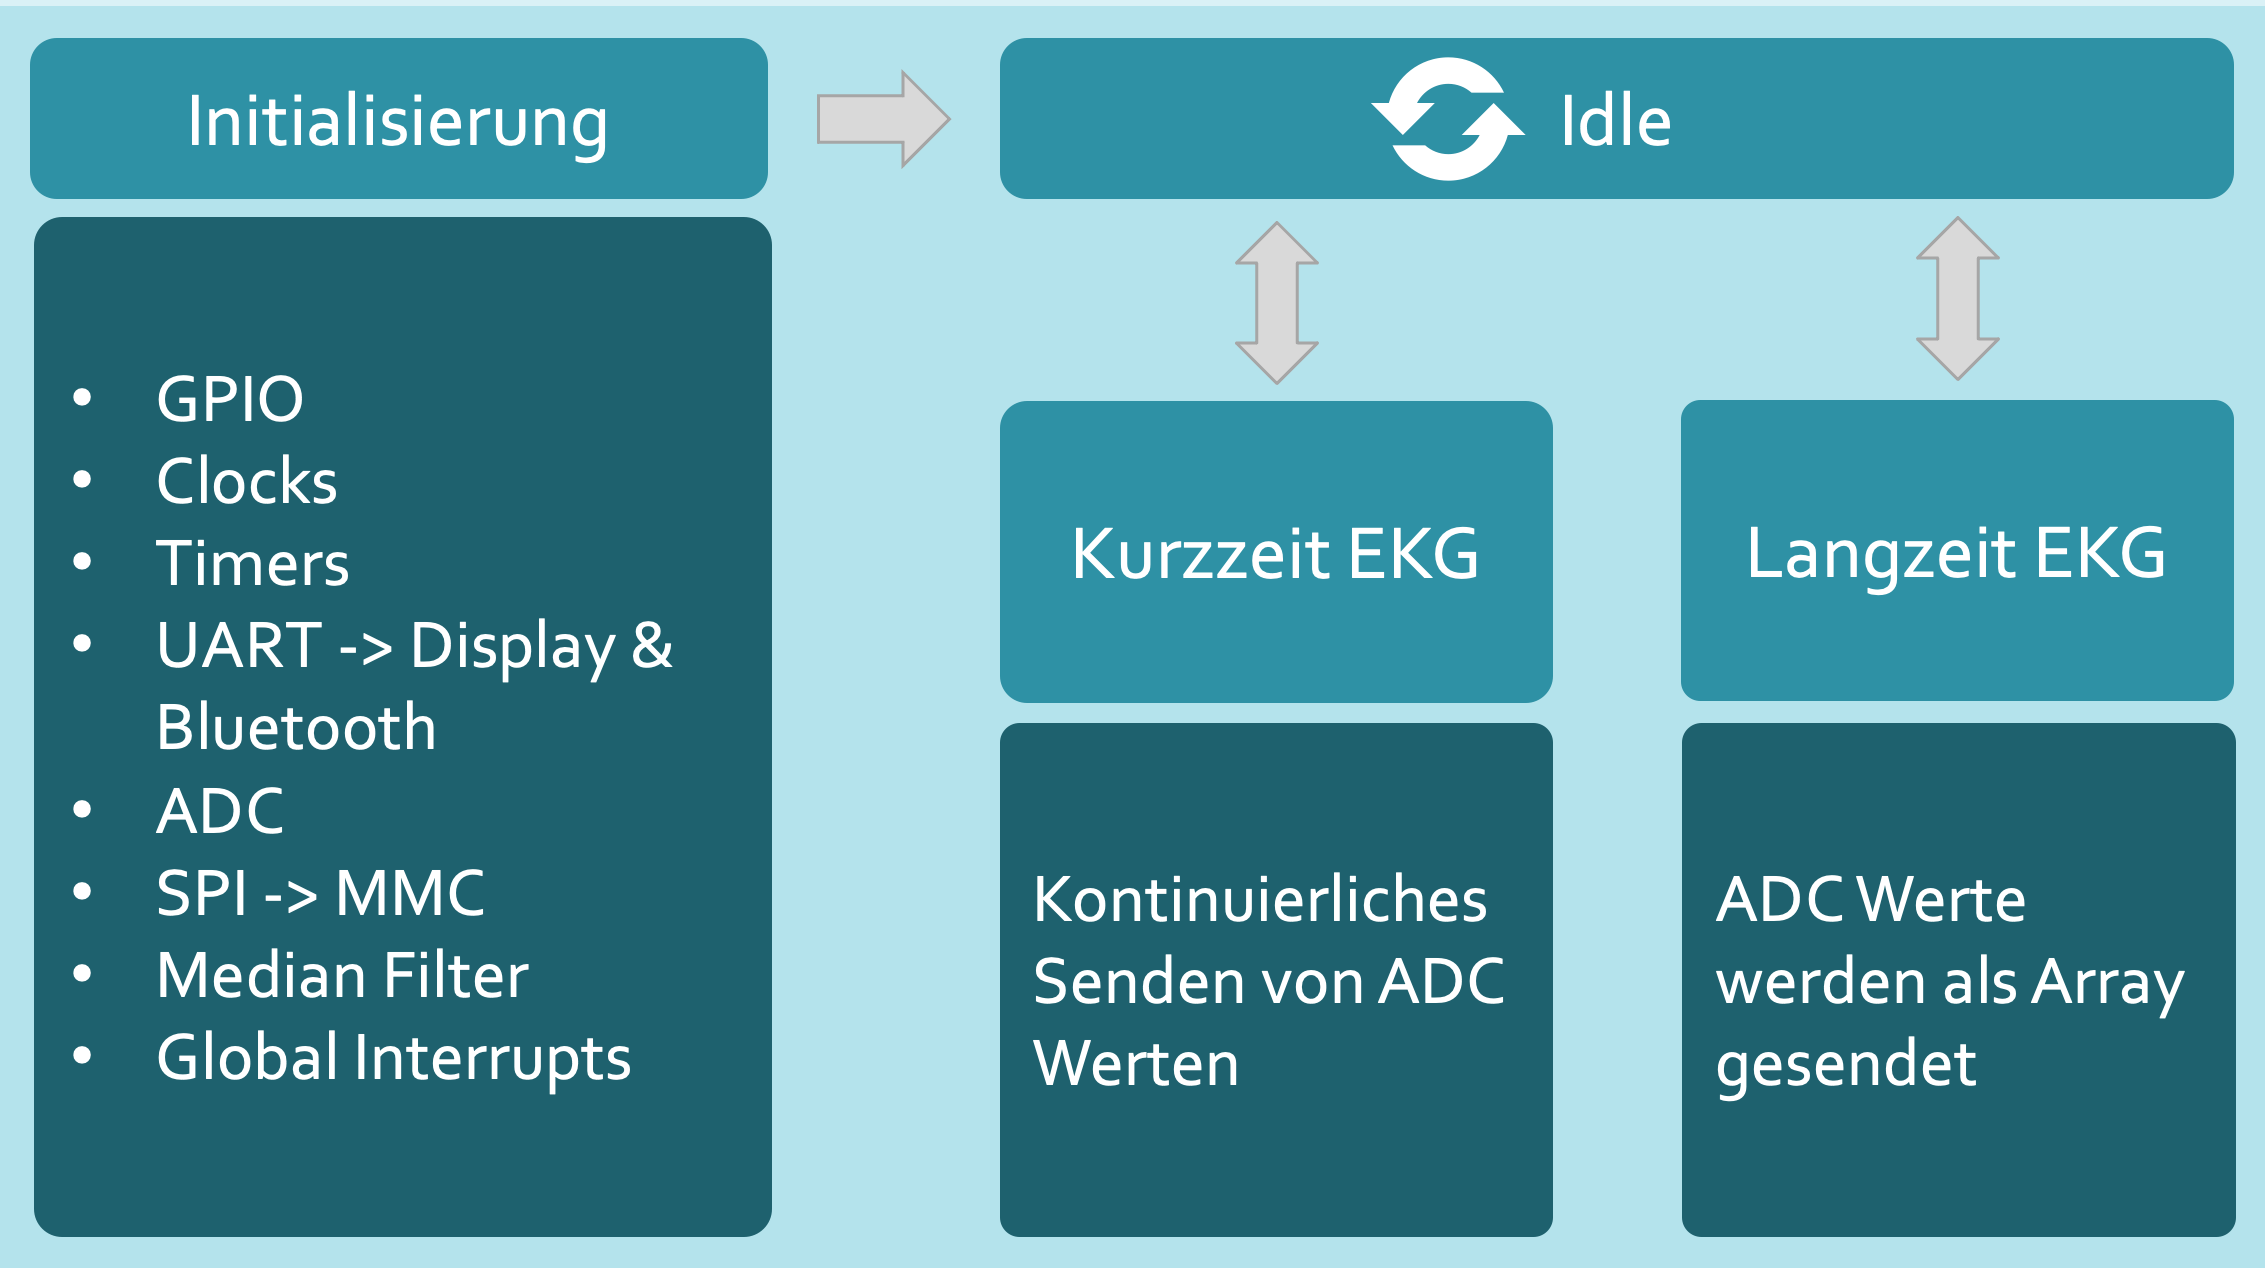
\includegraphics[width=12cm] {State Machine.png}
    \caption{State Machine des EKG7}
\end{figure}

Globale Flags: Für das Anzeigen diversen Zustände sind in der Software globalen Flags implementiert. Die Flags können folgende Ereignisse widerspiegeln:
\begin{itemize}
    \item Auftreten eines Interrupts,
    \item Ankommen von Daten,
    \item Aktueller Zustand der State Machine,
    \item Toggeln von der Taste,
    \item Zustände der Module,
    \item Timers,
    \item Bluetooth-Verbindung,
    \item Verbindung mit SD-Karte.
\end{itemize} 

Interrupts: Ein Interrupt ist ein Signal an die MCU, das hardware- oder softwareseitig auftritt und eine sofortige Antwort bzw. Reaktion der MCU benötigt. Der normale Programmablauf wird dabei gestoppt und es werden Befehle im Interrupt Service Routine erst ausgeführt. Nach dem Ablauf von einem Interrupt kehr die MCU zurück zum normalen Programmablauf.
In dem Projekt werden Interrupts für folgende Module verwendet:
\begin{itemize}
    \item GPIO – beim Togglen der Gehäusetaste, Ein- und Ausschalten des Bluetooth Moduls und Einsetzen bzw. Rausnehmen der SD-Karte,
    \item Timers – es treten zwei Interrupts auf mit jeweils 1 Hz und 250 Hz Frequenz,
    \item UART – beim Empfangen von Befehlen vom Display,
    \item ADC – beim Empfangen von EKG Signalen und Akkuspannung.
\end{itemize} 

Initialisierung: Initialisierung oder SYS\_INIT ist der Anfangszustand der MCU nach dem Einschalten. Dieser Zustand ruft Initialisierungsfunktionen aller verwendeten Modulen auf und nach dem Initialisierungsvorgang wird verlassen. Hier folgt die Reihenfolge der Module, die im Programm initialisiert werden:
\begin{itemize}
    \item Watchdog Timer – ist dem Totmann-Schalter ähnlich. Die MCU wird zurückgesetzt, wenn das Programm ihn nicht explizit ausschaltet;
    \item General Purpose Input Output – sind alle programmierbare MCU I/O Pins. Sie müssen vorerst initialisiert werden, da auf deren Funktionalität weitere Module basieren können;
    \item Clocks – Grundtaktfrequenz des Mikrocontrollers;
    \item Timers – Interrupts, die taktfrequenzabhängig sind und in gewissen Zeitintervallen auftreten;
    \item UART – Schnittstelle für Display- und Bluetooth-Verbindung;
    \item ADC – Digitalisierung der analogen Signale;
    \item SPI – Schnittstelle für Verbindung mit SD-Kartenmodul;
    \item FAT – File Allocation Table ist die Dateizuordnungstabelle bzw. ein Dateisystem für die Datenübertragung auf SD-Karte;
    \item UART-BT – Kommunikation der MCU mit dem Bluetooth Modul;
    \item Median Filter – Filterung der Artefakte bei der Herzfrequenzberechnung;
    \item Globle Interrupts – Freischalten der globalen Interrupts.
\end{itemize}

Im Folgenden wird eine detaillierte Beschreibung von den zu initialisierenden Modulen aufgelistet:
\begin{enumerate}
    \item GPIO: General Purpose Input Output ist ein Modul, das die vorhandenen Pins als Inputs oder Outputs initialisiert. Demnächst können diese Pins im Code verwendet werden. In diesem Modul werden folgende Pins initialisiert:
    \begin{itemize}
        \item LEDs auf dem PCB,
        \item Buzzer,
        \item 5V DC/DC,
        \item Gehäusetaste,
        \item Bluetooth State,
        \item Card Detect Pin für das SD-Kartenmodul.
    \end{itemize}
    \item Clocks: Es werden drei Clocks initialisiert. MCLK (Main Clock) und SMCLK (Sub-main Clock) weisen eine Frequenz von 20 MHz auf. ACLK (Auxiliary Clock) ist mit einer Frequenz von 32 kHz initialisiert.
    Main Clock wird als Taktquelle für die MCU verwendet. Sub-main Clock ist ein Hochfrequenztakt und wird für Peripheriemodule verwendet. Auxuliary Clock wird für Peripheriemodule verwendet, die einen niederfrequenten Takt benötigen.
    \item Timers: Im Code sind zwei Timers initialisiert. Timer A1 hat ACLK als Taktgeber und wird mit einer Frequenz von 1 Hz aufgerufen. Timer A2 ist an SMCLK gebunden und weist eine Frequenz von 250 Hz auf. Die zwei Timers funktionieren unabhängig voneinander und haben ihr eigenen ISR.
    \item UART Display: Bei der Initialisierung der UART Verbindung zum Display, werden zunächst die Input- (RX) und Output- (TX) Pins festgelegt. Die Frequenz der MCU beträgt 20 MHz. Als Baudrate wurde 115200 bps gewählt. Damit eine Verbindung der beiden Module besteht, muss die Baudrate sowohl beim Display als auch bei der MCU einprogrammiert werden. 
    Befehle vom Display an die MCU werden mittels Interrupts realisiert. Das Display sendet eine Folge zwischen vier und sieben Byte, welche im Nextion-Editor des Displays einzusehen sind. Für welche Funktionen und Buttons des Displays ein Interrupt geschickt werden soll, wird im Nextion-Editor des Displays programmiert. Sobald die MCU eine gesendete Interrupt-Folge erkennt, werden Flags gesetzt. Anhand dieser Flags werden im späteren Verlauf gewisse Funktion auf der MCU aufgerufen.
    Bei Befehlen, die von der MCU an das Display gesendet werden, wird im Wesentlichen mit drei Funktionen gearbeitet. Bei der ersten Funktion wird ein Command mit der entsprechenden Variablen als String (z.B. „page0.akku.val“ – Bedeutung siehe Baugruppe Display und Benutzeroberfläche) an das Display gesendet. Mit der zweiten Funktion wird der dazugehörende Wert, z.B. akku\_percentage, der Integer Werte in einen String umgewandelt und anschließend an das Display sendet. Um einen Befehl auch als solchen zu, erwartet das Display drei Bytes mit dem Inhalt „0xFF“ am Ende. Diese drei Byte werden in der dritten und somit letzten UART-Funktion an das Display gesendet. Anhand dieser drei Funktionen ist die Kommunikation fertiggestellt.
    \item UART Bluetooth-Modul: Das verwendete Bluetooth Modul HC-05 wird über UART angesprochen, wobei die Baudrate flexibel konfigurierbar ist. Zum Transfer von Daten öffnet das Modul auf dem verbundenem Smartphone oder Laptop einen virtuellen COM-Port, über welchen es alle ihm übergebenen Bytes ausgibt. Seitens der MCU wird das Hardware-Modul USCI\_A1 verwendet, welches mit Ausnahme der Basisadresse identisch zu USCI\_A0 bzw. Display initialisiert wird.
    Um beim versenden der Nachrichten keine Verzögerung oder zusätzliche CPU Last zu verursachen, wird Direct Memory Acces (DMA) verwendet. Das DMA-Modul kann nach korrekter Initialisierung automatische Daten im Hintergrund in das TX Register des UART Moduls kopieren. Hierfür muss das Modul auf Single Transfer konfiguriert werden. Weitere benötigte Konfigurationen sind Byte-to-Byte Transfer, die Quelladresse, die Zieladresse und die Datengröße. Als Trigger um das nächste Byte zu übertragen ist das Interrupt Flag UCA1TXIFG zu wählen, welches immer dann aktiv ist, wenn das UART Modul bereit ist ein weiteres Byte zu senden. Damit ein ganzer String verschickt werden kann, ist das DMA Modul auf ein Inkrementieren der Quelladresse nach jedem versendetem Byte einzustellen. Somit wird nach Aktivierung des Moduls durch setzen des DMA-Enable-Bits ein kompletter String im Hintergrund Byte für Byte versendet, bis die vorgegebene Datengröße abgearbeitet ist und das Enable-Bit automatisch zurückgesetzt wird. Die CPU selbst wird dabei jeweils nur für zwei Takte durch das DMA Modul unterbrochen und muss nicht auf den Abschluss jedes Sendevorgangs warten.
    \item ADC: Demnächst wird das ADC Module initialisiert. Als Referenzspannung wird 1,5 V gesetzt. Das ist ein Standardwert. Als nächstes werden zwei Pins für EKG Aufnahme und Akkubeobachtung initialisiert. Als positive Referenzspannungsquelle wird AVCC (3V) für beide ADC Kanäle eingestellt. Negative Referenzspannungsquelle ist AVSS, was dem Groundpotential auf dem PCB entspricht. Beide Kanäle werden mit ACLK betrieben. Zum Schluss wird ein Interrupt für dieses Modul und das Modul selbst aktiviert.
    \item SPI: Die SPI Schnittstelle wird mit einem SMCLK betrieben und kann die maximale Frequenz von 20 MHz erreichen. Nach dem Konfigurieren von Grundfrequenz und gewünschter Frequenz wird das SPI Modul aktiviert, Interrupt freigeschaltet, das Signal Chip Select gesendet und TX Buffer aktiviert. Wenn TX Buffer aktiv ist, wird ein Wert „0x00“ an Slave gesendet. 
    \item FAT: FAT ist eine SPI-basierte Schnittstelle und benutzt SPI als Kommunikationsprotokoll. FAT Modul initialisiert SD-Karte. Dafür wird in diesem Projekt eine Open Source Library FatFs der Entwickler elm-chan.org verwendet. Diese Library ist unter „Creative Commons Attribution 3.0 Unported License“ lizenziert und daher kann für nichtkommerzielle Zwecke benutzt werden. 
    SD-Karte wird mit einem Timeout initialisiert, was nicht nur das Detektieren der Karte im Kartenmodul ermöglicht, sondern auch das Testen von den Lese- und Schreibvorgängen. Somit kann geprüft werden, ob die SD-Karte funktionsfähig ist.
    \item Medianfilter: Um Artefakte bei der Herzfrequenzmessung herauszufiltern, dient ein Medianfilter. Bei der Initialisierung werden zwei Strukturen und ein Array der Größe 11 angelegt. Ein Medianfilter gibt immer den Wert zurück, der sich in der Mitte des Arrays befindet. Anders als bei einem Mittelwertfilter, haben größere Artefakte keinen Einfluss auf den Medianwert. Dadurch wird sichergestellt, dass die Herzfrequenzmessung auch beim Aufstehen des Patienten oder großen Störfaktoren richtig berechnet wird. Aufgerufen wird die Median-Funktion unmittelbar nach der Herzfrequenzberechnung. In dem Array werden 11 Werte gespeichert und stets der Medianwert an das Display übermittelt.
\end{enumerate}

IDLE State: Direkt nach dem Initialisierungsvorgang der MCU, befindet man sich im IDLE\_STATE. 
Als IDLE\_STATE wird der Zustand bezeichnet, in dem sich das EKG-Gerät im Leerlauf befindet. Hier wird kontinuierlich in einer while-Schleife abgefragt, ob der Benutzer/die Benutzerin ein Kurzzeit- oder Langzeit-EKG aufnehmen möchte.
Eine erfolgreiche Abfrage wird durch den Start-Befehl des Displays in Form eines Interrupts erreicht. Sobald der Benutzer/die Benutzerin den Befehl gibt, wird eine CSV Datei auf der SD-Karte erstellt und der Case der State Machine wechselt entsprechend der gewünschten Aufnahme Methode.

Kurzzeit-EKG aus Nutzersicht: Im Falle einer Kurzzeit-Aufnahme startet man das EKG auf dem Display im Unterpunk „Kurzzeit EKG“. Sobald dieser Befehl ausgeführt wurde, läuft die Aufnahme samt Speicherung für zwei Minuten automatisch ab. Um das EKG vorzeitig abzubrechen, kann der Stopp-Button des Displays betätigt werden. Dabei ist eine Sicherheitsabfrage vorzufinden, ob der Befehl bewusst oder unbewusst getätigt wurde. Gestoppt wird somit erst nach der Bestätigung auf „Ja“. Ansonsten läuft die Aufnahme bis Vollendung der zwei Minuten weiter.
\begin{figure} [!h]
	%\centering
	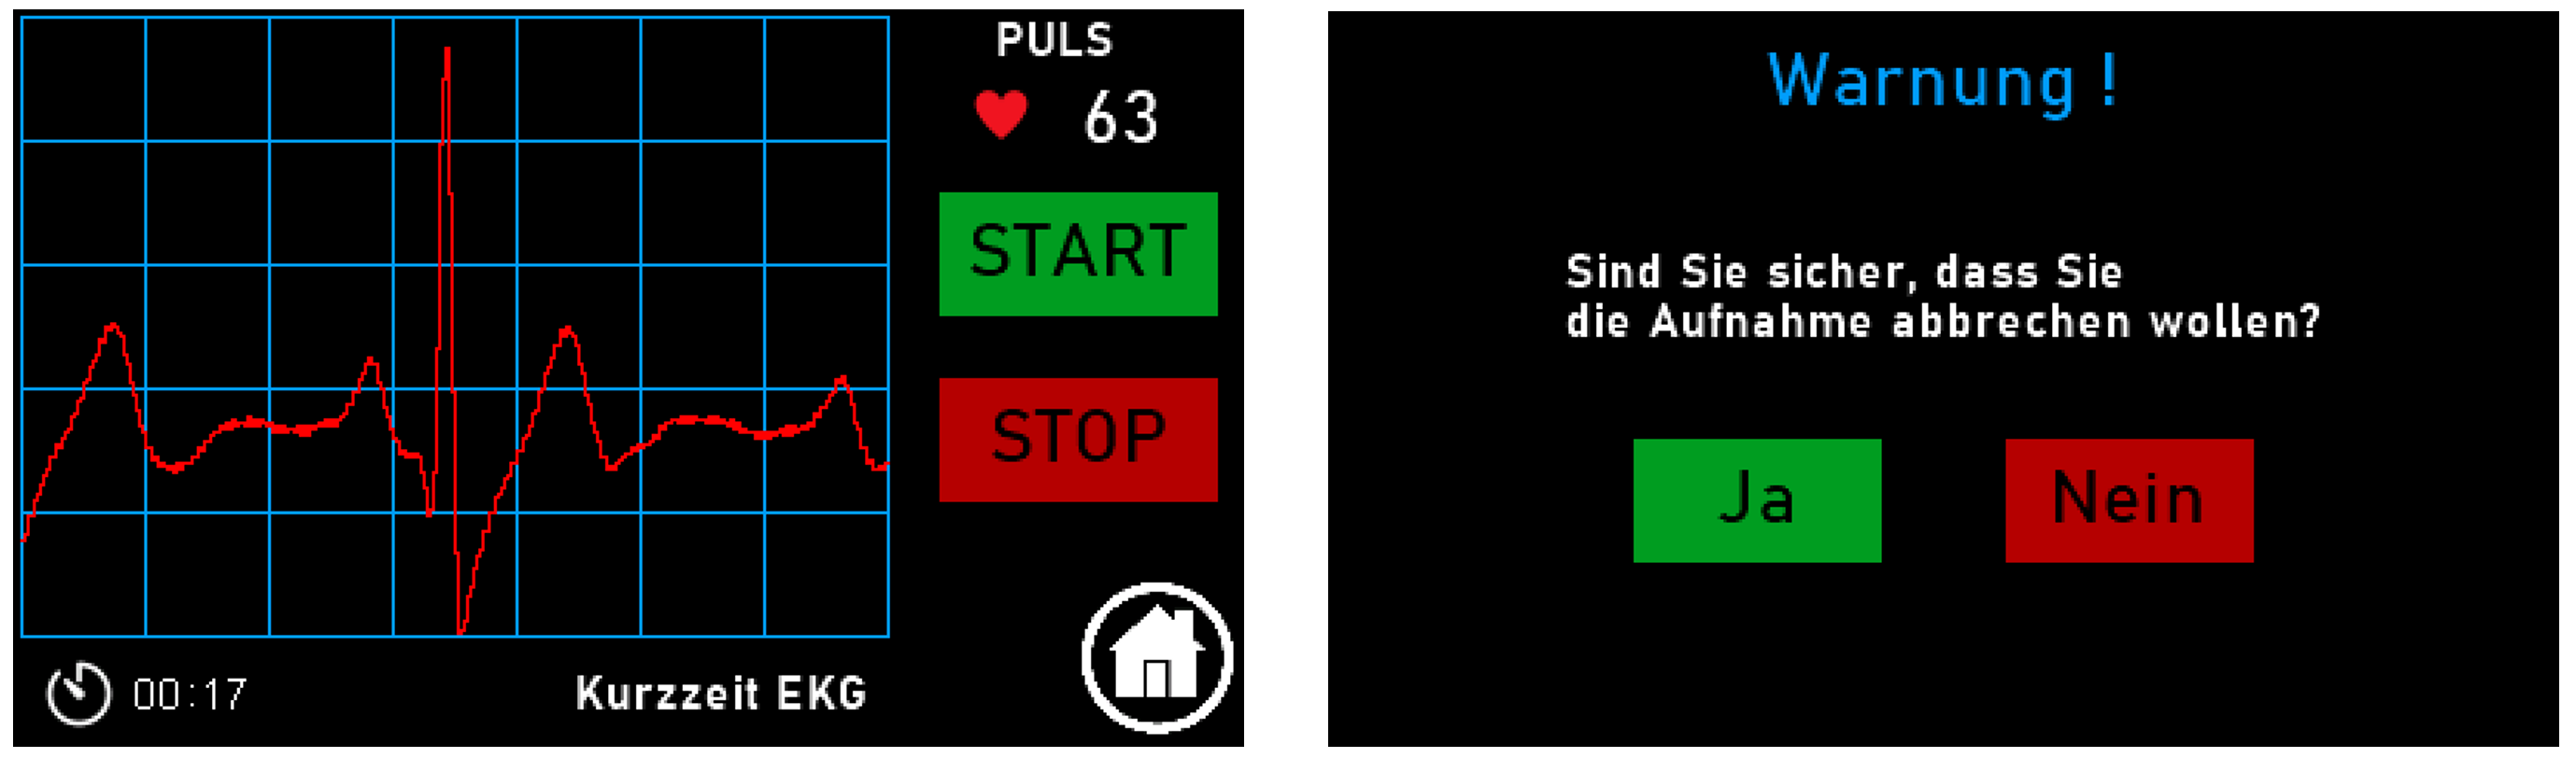
\includegraphics[width=\textwidth] {Short ECG.png}
	\caption{Display UI einer Kurzzeit-Aufnahme}
\end{figure}

Langzeit-EKG aus Nutzersicht: Im Gegensatz zum Kurzzeit-EKG, weist das Schema einer Langzeit-Aufnahme einige Änderungen auf. Gestartet wird ebenfalls durch einen Start-Befehl auf dem Display. Hier ist jedoch zu beachten, dass der Ladestand der Batterie beim Start mindestens 80 \% aufweist. Eine Aufnahme ist ansonsten nicht möglich, da es im Falle eines zu leeren Akkus zu Datenverlust kommen kann. Bei der Langzeit-Aufnahme läuft das EKG für 24 Stunden automatisch. Um eine Aufnahme über 24 Stunden gewähr zu leisten, muss der Nutzer/die Nutzerin den Power Button des Geräts einmalig drücken. Dadurch wird der Stromsparmodus aktiviert und das Gerät wechselt automatisch zwischen einem ON- und OFF-Modus. Im OFF-Modus ist die 5 V Peripherie (das Display und das Bluetooth-Modul) vollständig deaktiviert. Der ON-Modus hingegen, aktiviert alle vier Sekunden das SD-Kartenmodul und speichert die gesammelten Werte in der CSV Datei ab. Bei erneutem Betätigen des Power Buttons wird der Stromsparmodus verlassen und der Zugriff auf das Display wieder gewährt. Um die Aufnahme vorzeitig abzubrechen, kann der Stopp-Button auf dem Display betätigt werden. Wie auch beim Kurzzeit-EKG wird durch die Sicherheitsabfrage ein unbewusstes Drücken verhindert.

Energy Saving Mode Nutzersicht: Um ein schnelles Entladen der Batterie entgegenzuwirken und eine möglichst lange Lagerung (Shelf-Time) zu garantieren, verfügt das EKG-Gerät über einen Energiesparmodus. Die MCU befindet sich während diesem Vorgang im ENERGY\_SAVING\_MODE. Um diesen zu aktivieren, wird im IDLE\_STATE der physische Button am Gehäuse gedrückt, der die gesamte 5 V Peripherie abschaltet. Beim Betätigen des Tasters, sind drei akustische Töne eines Buzzers zu hören.

Wakeup Mode Nutzersicht: Um den Energiesparmodus wieder zu verlassen, gibt es den Case SYS\_WAKEUP. Aufgerufen wird dieser, wenn während dem Energiesparmodus der Button am Gehäuse gedrückt wird. Die gesamte 5 V Peripherie schaltet sich dabei an und das akustische Signal des Buzzers ist erneut zu hören.

Akku-, BT-, SD-Abfrage: Abgesehen von der State Machine, befindet sich noch eine if-Abfrage in der main Funktion. Dabei handelt es sich um drei Funktionen, die jede Sekunde im IDLE\_STATE oder während einer Kurz- / Langzeitaufnahme ausgeführt werden.
\begin{itemize}
    \item ADC\_Akku\_Average\_Value berechnet alle drei Sekunden den Mittelwert der ADC-Werte, welche am Akku anliegen. Anhand des Mittelwertes wird der Akku in Prozent umgerechnet. Somit ist das Ablesen des Ladestandes auf der Startseite für den Benutzer/die Benutzerin intuitiv und einfach zu verstehen.
    Der Prozentbetrag wird jede dritte Sekunde auf dem Display aktualisiert.
    \item Check\_BT\_Connection und Check\_SD\_Card\_Connection sind zwei Funktionen, die die aktuelle Verbind der Peripherie zum Bluetooth Modul und zum SD-Kartenleser auf dem Display anzeigt. Es werden die State-Pins der Module abgefragt und ein Symbol auf das Display gesetzt. Wenn die Verbindung steht, sind die Symbole auf der Startseite blau. Bei keiner Verbindung werden die Symbole grau.
    \item Bei der Abfrage für die SD-Karte gibt es außerdem zwei zusätzliche Funktionen. Wenn die SD-Karte herausgezogen wird, erscheint auf dem Display eine Warnmeldung. Die Speicherung bei einem Langzeit-EKG erfordert eine eingelegte SD-Karte. Beim Entfernen und wieder Anschließen einer SD-Karte, wird diese neu initialisiert und die aktuellen Daten bleiben vorhanden.
\end{itemize}

Aufnahme eines Kurzzeit-EKG: Die Kurzzeit-EKG Aufnahme wird kontinuierlich durchgeführt. D.h. die ADC Werte werden direkt an das Display und SD-Karte übertragen ohne Zwischenspeichern. Nachdem die MCU auf ECG\_SHORT Zustand wechselt, wird als erstes ein Timer auf dem Display gestartet. Der Timer zählt, wie lange die EKG Aufnahme durchgeführt wird. Nach zwei Minuten wird die Aufnahme automatisch beendet und der Benutzer wird benachrichtigt. Zunächst wird es auf 250 Hz Flag gewartet und sobald die Flag ungleich Null ist, wird ein ADC Wert aufgenommen und die Flag wird zurückgesetzt. Wenn ein neuer ADC Wert ankommt, wird eine weitere Flag gesetzt und dadurch wird der aufgenommene ADC Wert an das Display gesendet und demnächst auf die SD-Karte gespeichert. Die Flag wird zurückgesetzt.
Es wird durchgehend kontrolliert, dass es nur Kurzzeit-EKG aufgenommen wird. Sollte der Benutzer während der Aufnahme versuchen auf Langzeit-EKG zu wechseln, wird eine Warnung gezeigt und der Vorgang verhindert.
Nach der Aufnahme wird die Flag für Kurzzeit-EKG zurückgesetzt, die Datei auf der SD-Karte gespeichert, die Timer zurückgesetzt und die MCU geht in Idle Zustand. Das Display wird dementsprechend die Hauptseite anzeigen.

Aufnahme eines Langzeit-EKG: Im Gegensatz zu Kurzzeit-EKG, werden die Daten während der Langzeit-EKG Aufnahme intern auf der MCU gespeichert und blockweise in gewissen Zeitintervallen an SD-Karte gesendet. Da das SD-Kartenmodul an 5V angeschlossen ist und im Stromsparmodus 5V Peripherie komplett abgeschaltet ist, weicht die Logik von Kurzzeit-Aufnahme ab.
Beim Wechseln auf Langzeit-EKG Modus wird als erstes die Timer- und ADC-Werte an das Display gesendet. Somit kann der Benutzer den Kurvenverlauf und Dauer der Aufnahme sehen. Weiterhin wird die Stromsparmodus-Logik aufgerufen. Diese Logik enthält eine State Machine mit drei Zuständen. Die State Machine ist mit einer switch-Anweisung realisiert. Die drei Zustände sind: normaler Zustand (MODE\_NORMAL), 5V Peripherie an (MODE\_5V\_ON) und 5V Peripherie aus (MODE\_5V\_OFF). 
Die zwei Modi für 5V an und aus sind für Stromsparmodus entwickelt. Das Funktionsprinzip des Stromsparmodus ist auf dem Bild zu sehen.
\begin{figure} [!h]
	\centering
	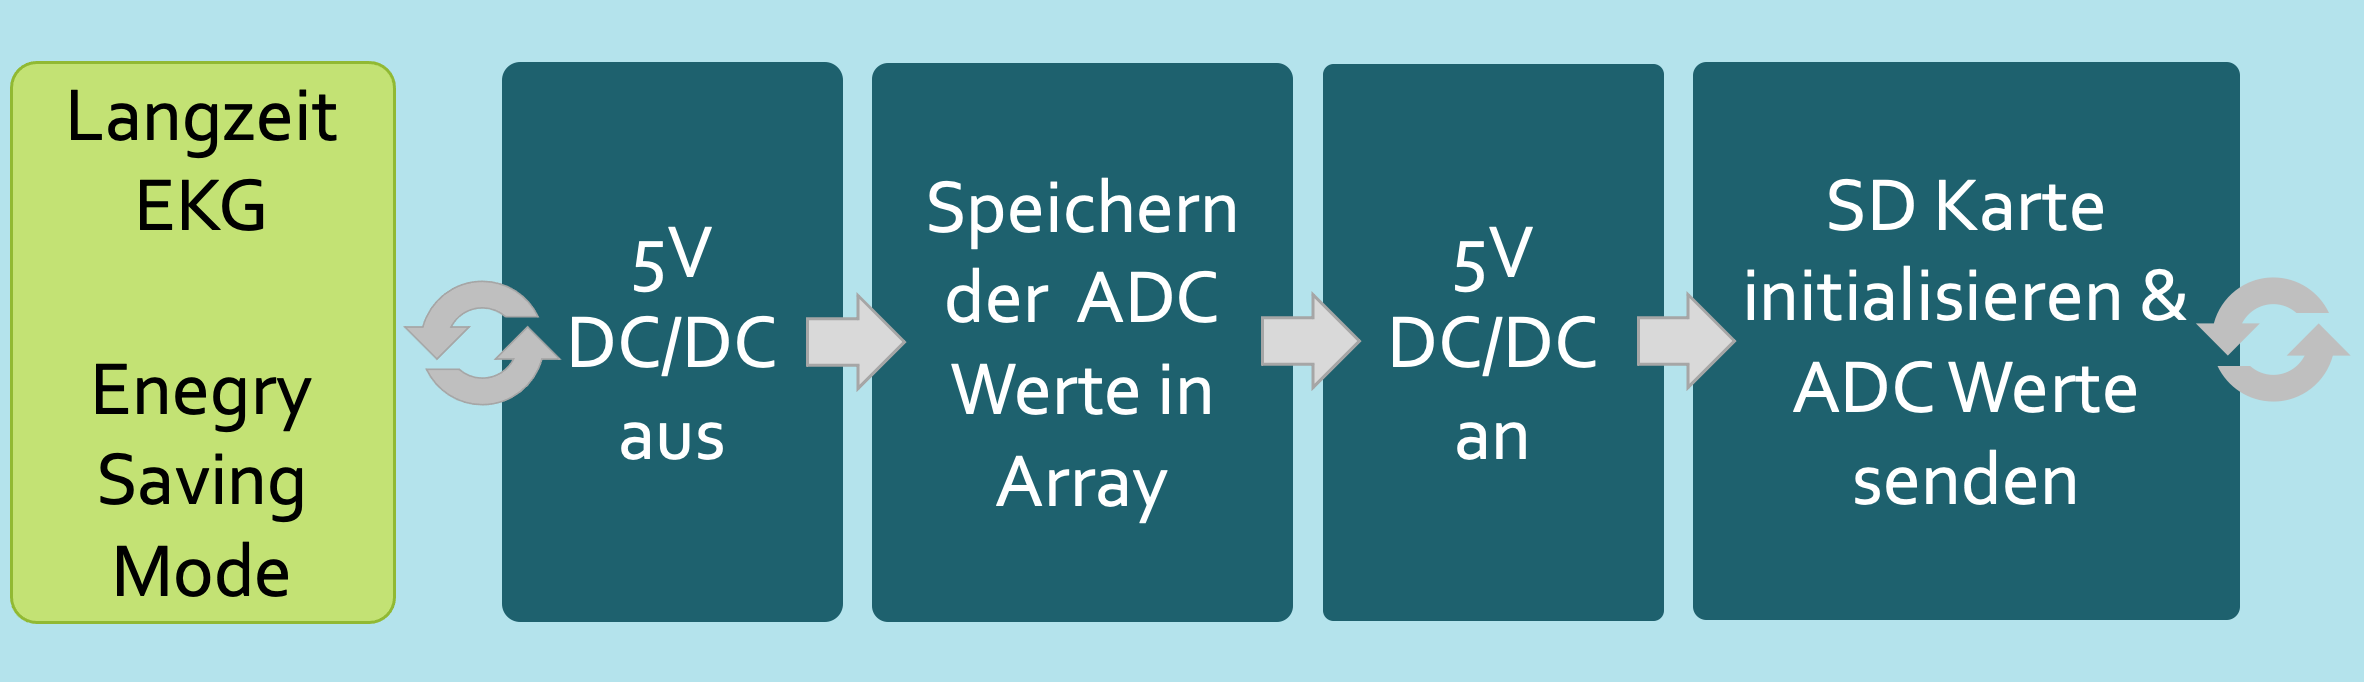
\includegraphics[width=12cm] {Langzeit EKG Energy Saving.png}
	\caption{Energy Saving Mode während Langzeit-EKG}
\end{figure}
Wenn der Benutzer 24 Stunden Aufnahme macht, ist es sinnvoll Energie zu sparen. Im Stromsparmodus wird die ganze 5V Peripherie komplett abgeschaltet, d.h. das Display, Bluetooth und SD-Karte werden nicht mehr versorgt. Das Stromsparmodus kann aktiviert werden, wobei der Benutze den Power Button auf dem Gehäuse einmal betätigt.
Wenn der Benutzer eine Langzeit-EKG Aufnahme gestartet hat, landet das Programm in MODE\_NORMAL zuerst und bleibt in diesem Zustand solange, bis der Benutzer den Power Button betätigt. Im normalen Zustand bleibt die ganze 5V Peripherie an, das QRS Komplex ist auf dem Display zu sehen und die ADC-Werte werden via Bluetooth gesendet. Der einzige Unterschied ist das Schreiben auf SD-Karte. Dieser Vorgang ist komplett verarbeitet und ist folgendermaßen realisiert. Es sind zwei Arrays mit jeweils 1000 Werten benutzt. Dadurch, dass ADC an 250Hz Timer gebunden ist, wird dieses Array innerhalb von 4 Sekunden aufgefüllt. Um sie zu unterscheiden, werden sie Main Storage und Redundant Storage genannt. Im ADC Interrupt wird jeder neue ADC-Wert in Main Storage gespeichert, und zwar so lange, bis das Array voll wird. Nachdem das Main Storage voll ist, wird das ganze Array in Redundant Storage kopiert. Somit kann Main Storage wieder überschrieben werden und währenddessen bleibt Redundant Storage unverändert. Wenn Main Storage voll ist und in Redundant Storage kopiert, wird eine Flag gesetzt und somit das Senden an SD-Karte gestartet. Nachdem das Senden fertig ist, wird der ganze Vorgang wiederholt.
Wenn der Power Button betätigt wird, geht die MCU aus dem MODE\_NORMAL in MODE\_5V\_OFF. In diesem Zustand wird 5V Peripherie abgeschaltet. Der Zustand kann verlassen werden, wenn entweder Main Storage voll ist und entsprechende Flag gesetzt ist, oder der Power Button nochmal betätigt wird.
Wenn die Flag gesetzt wird, geht die MCU in MODE\_5V\_ON in dem die 5V Peripherie wieder versorgt wird. Demnächst wird die SD-Karte initialisiert und das bereits kopierte Redundant Storage an die SD-Karte geschrieben. Danach geht die MCU in MODE\_5V\_OFF und der Vorgang wird wiederholt.
Wenn der Power Button betätigt wird, geht die MCU in MODE\_NORMAL, zeigt die Werte auf dem Display und sendet Daten via Bluetooth bei Bedarf. In diesem Zustand kann der Benutzer entweder die Aufnahme beenden oder das Gerät wieder in Energy Saving Mode senden. 
Die Aufnahme wird nach 24 Stunden automatisch beendet und die MCU geht wieder in Idle State.

Energy Saving Mode und Wakeup Mode (Code): Das EKG-Gerät verfügt über einen physischen Button, der die 5 V Peripherie steuert. Dadurch wird das Gerät in einen Energiesparmodus versetzt um eine lange Lagerung zu ermöglichen.
Beim Drücken des Buttons, wird ein Interrupt im GPIO verursacht. Mithilfe einer Delay-Funktion wird auf das Entprellen der Taste geachtet. Im Interrupt wird eine 5V-Flag gesetzt. Diese Flag ist mit „FALSE“ initialisiert. „FALSE“ bedeutet demnach, dass die 5 V Peripherie eingeschaltet ist.
Beim erstmaligen drücken wird die Flag auf „TRUE“ gesetzt. Dabei gelangt man in den Case ENERGY\_SAVING\_MODE. In diesem Case wird eine Funktion aufgerufen, die den 5 V DCDC abschaltet. In dieser Funktion wird zunächst die Buzzer-Funktion gestartet. Der Buzzer wird drei Mal mir einer Frequenz von 250 Hz angeregt und generiert dadurch drei akustische Töne. Nachdem der Nutzer das akustische Signal bekommen hat, wird die gesamte 5 V Peripherie abgeschaltet. Da der Pin, der den Status der SD-Karte wiedergibt mit 3 V betrieben wird, wird abgefragt ob sich die SD-Karte im Gerät befindet. Dementsprechend wird eine weitere Flag gesetzt.
Bei erneutem Drücken des Buttons wird wieder ein Interrupt ausgelöst, der nun die 5V-Flag zurück auf „FALSE“ setzt. Dabei gelangt man in den Case SYS\_WAKEUP. In diesem Case wird die Funktion State\_sys\_Wakeup\_Mode ausgeführt. Die gesamte 5V Peripherie wird wieder angeschaltet. Nachdem der Buzzer das akustischen Signale nach dem Anschalten wiedergibt, gelangt die MCU zurück in den IDLE\_STATE. Die Flag, welche beim Ausschalten für die SD-Karte gesetzt wurde, wird nun durch Check\_SD\_Card\_Connection in der main Funktion abgefragt. Demnach wird auf dem Display die Verbindung angezeigt.
\begin{figure} [!h]
	\centering
	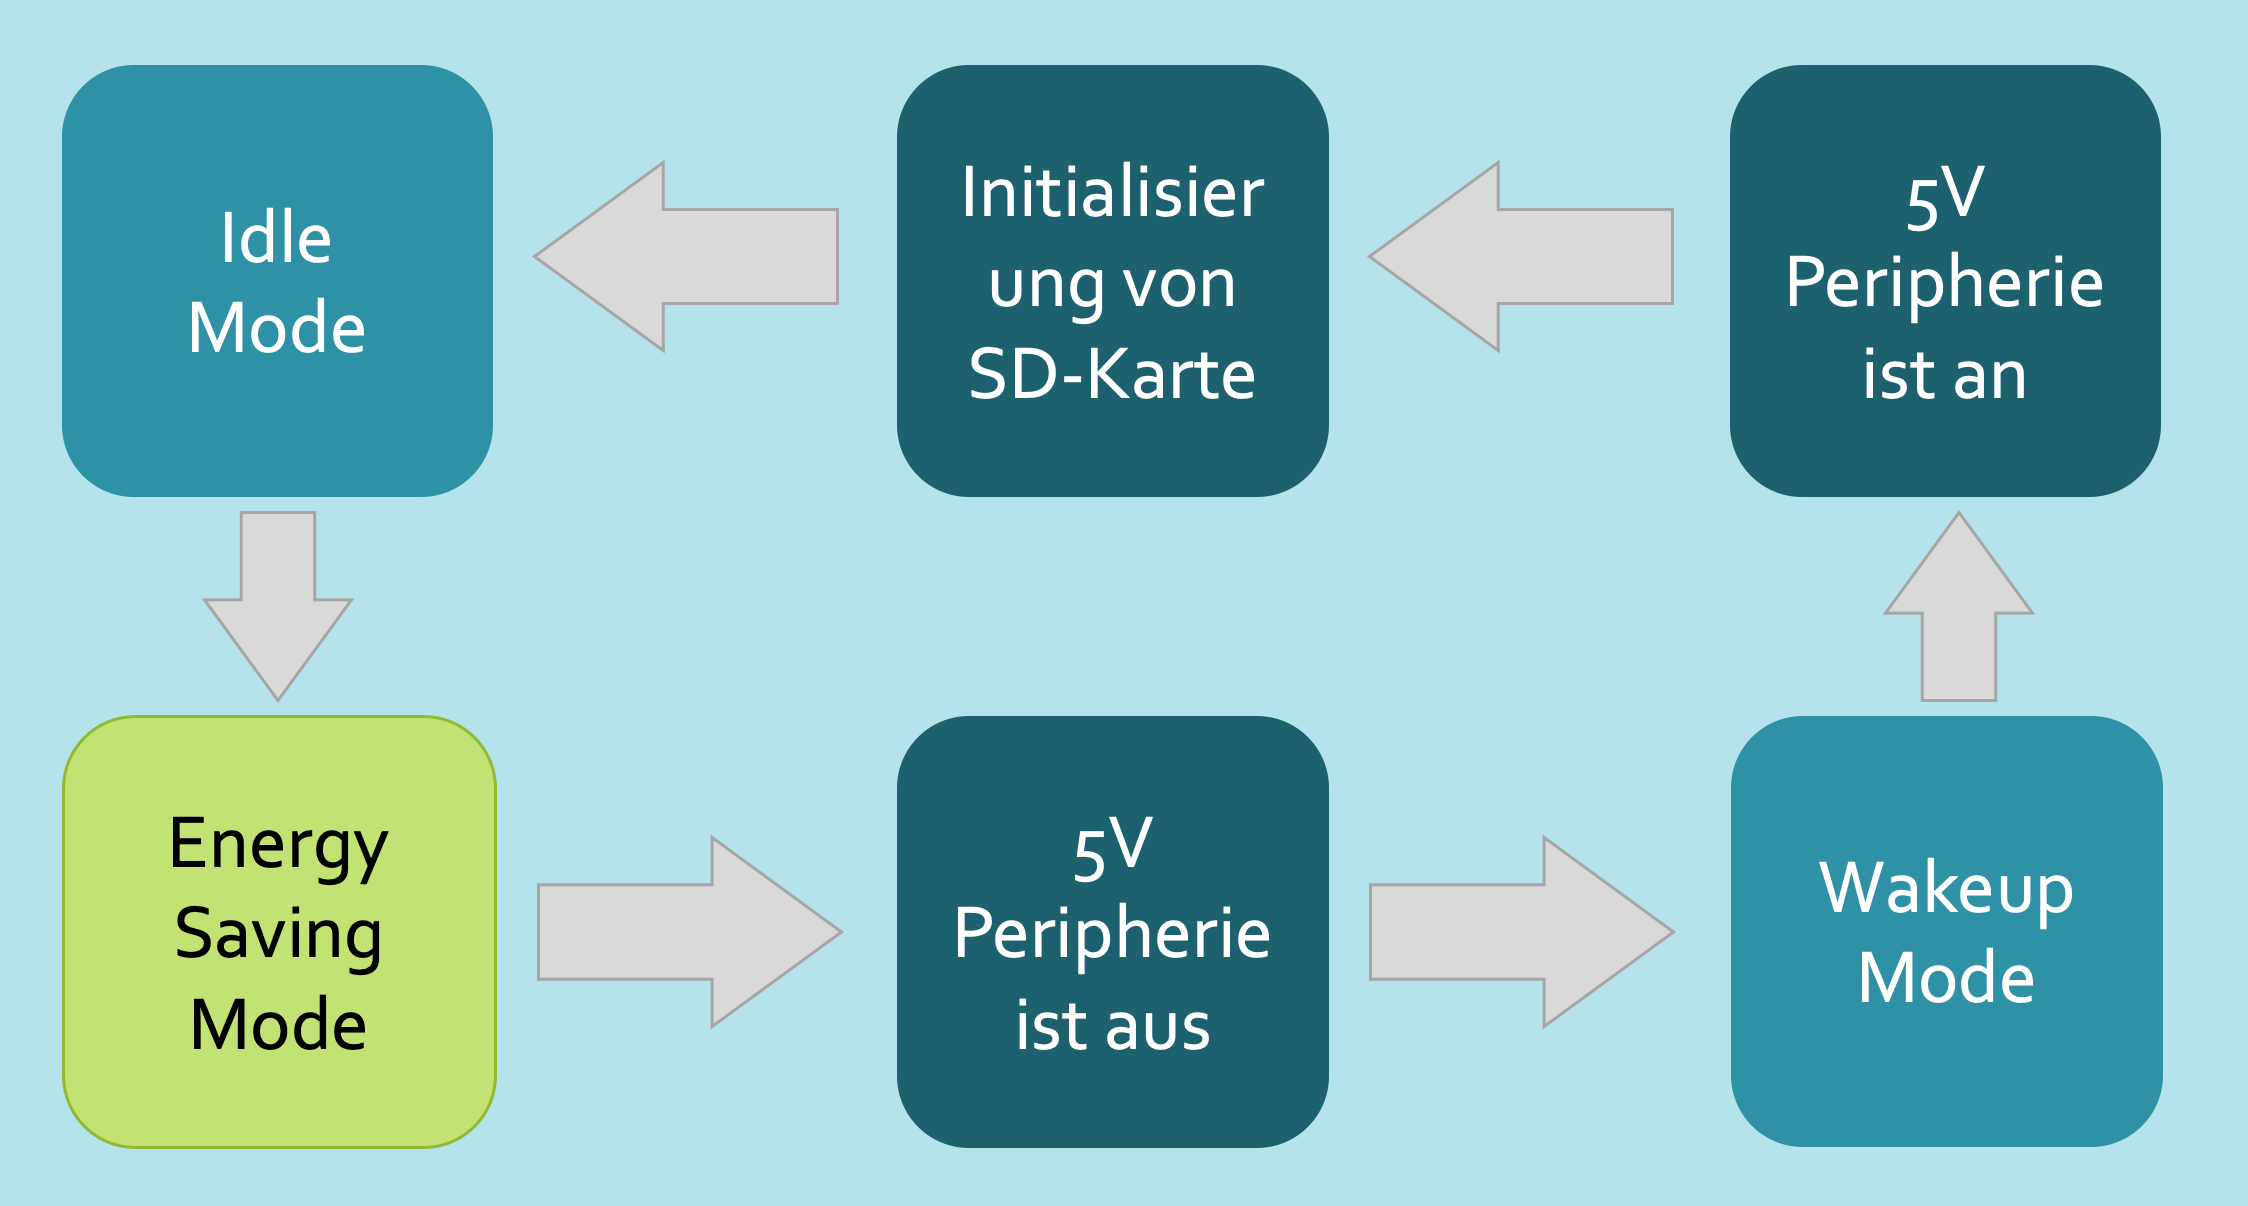
\includegraphics[width=12cm] {Idle State and Evergy Saving.png}
	\caption{Energy Saving Mode in Idle State}
\end{figure}